\chapter{Nuclear Models}

\section{Introduction}

In the following, it is worth to make a discussion about the nuclear models that are used by theoreticians in order to describe phenomena that are specific to rotating nuclei and high-spin regime. Since the focus of this work emerges from a \emph{class} of properties that usually apply to the high-spin region (but this does not necessarily also imply a high-energy region), it makes sense to give an insight in the tools that fit the best the underlying effects.

\subsection{Shell model}

The fact that an atomic nucleus can have a structure that behaves rather similarly as its \emph{parent} (i.e., the atom) in terms of changing the number of constituents, has been enforced by the experimental observations that were done across time. The sharp and discrete discontinuities of nuclear properties, such as the nucleon separation energy, point to the fact that nucleus can be explained through the existence of \emph{shells}. Some examples of observations which indicate this are:
\begin{itemize}
    \item When adding a nucleon to a nucleus, there are certain places where the \emph{binding energy} of the next nucleon becomes considerably smaller than the previous one. 
    \item Separation energies for both the protons and neutrons suffer drastic changes, having strong deviations from the predictions of the semi-empirical mass formula \cite{weizsacker1935theorie}, the discontinuities being represented by major shell closures (complete filling) \cite{krane1991introductory}.
    \item The neutron absorption cross-section has a substantial decrease in value at the neutron magic numbers
    \item Great abundance of nuclides where $Z$ and $N$ are magic numbers.
\end{itemize}

The sudden discontinuities occur at specific values of the proton $Z$ and neutron $N$ numbers: these are called \emph{magic numbers}. Currently, these magic numbers correspond to $Z$ or $N=2,8,20,28,50,82,126$, and they represent the so-called major shells. There are also two \emph{weakly magic numbers}: 40 and 64.

One can examine the values for the first excited states $2^+$ that are shown in Figs. \ref{e2plus_proton}-\ref{e2plus_neutron}. Indeed, these values show some peaks, each peak corresponding to a particular magic number.

\begin{figure}
    \centering
    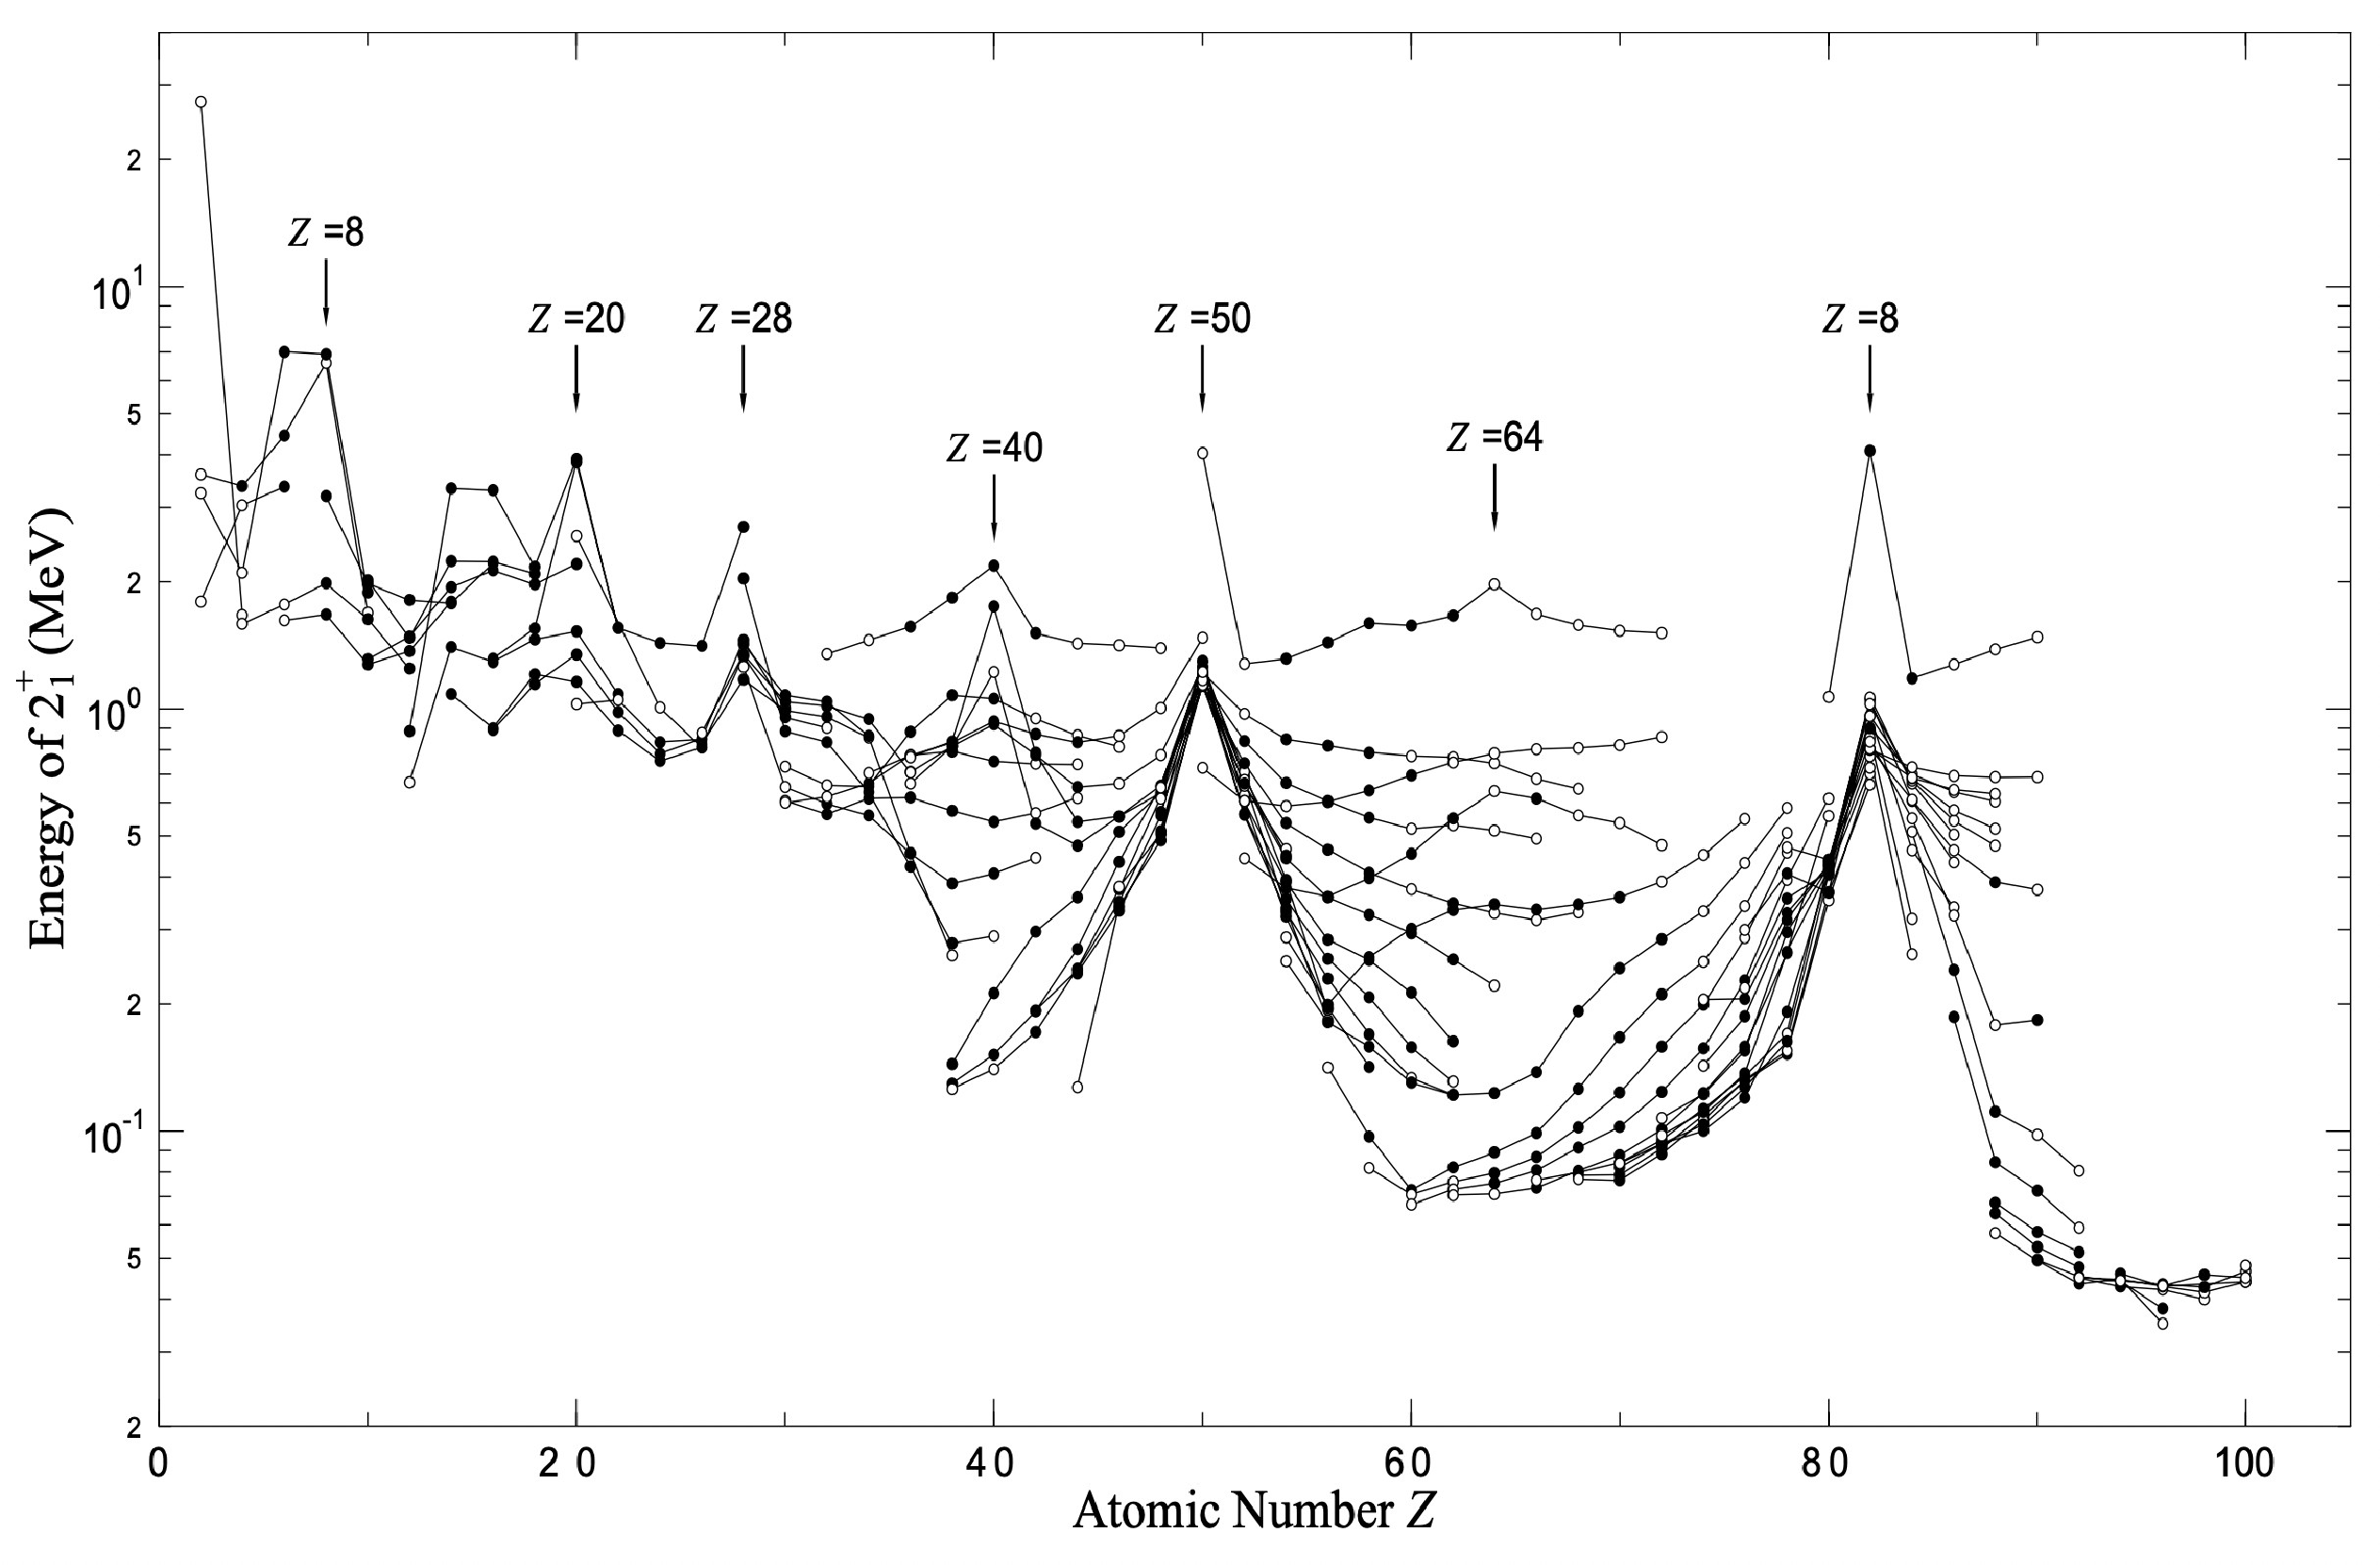
\includegraphics[scale=0.3]{Chapters/Figures/E2plus_proton.pdf}
    \caption{The first excited energy states $2^+$ of nuclei with even $Z$ and $N$ graphically represented with respect to the proton number. Each line represents a set of isotopes. Figure taken from Ref. \cite{matta2017exotic}}.
    \label{e2plus_proton}
\end{figure}

\begin{figure}
    \centering
    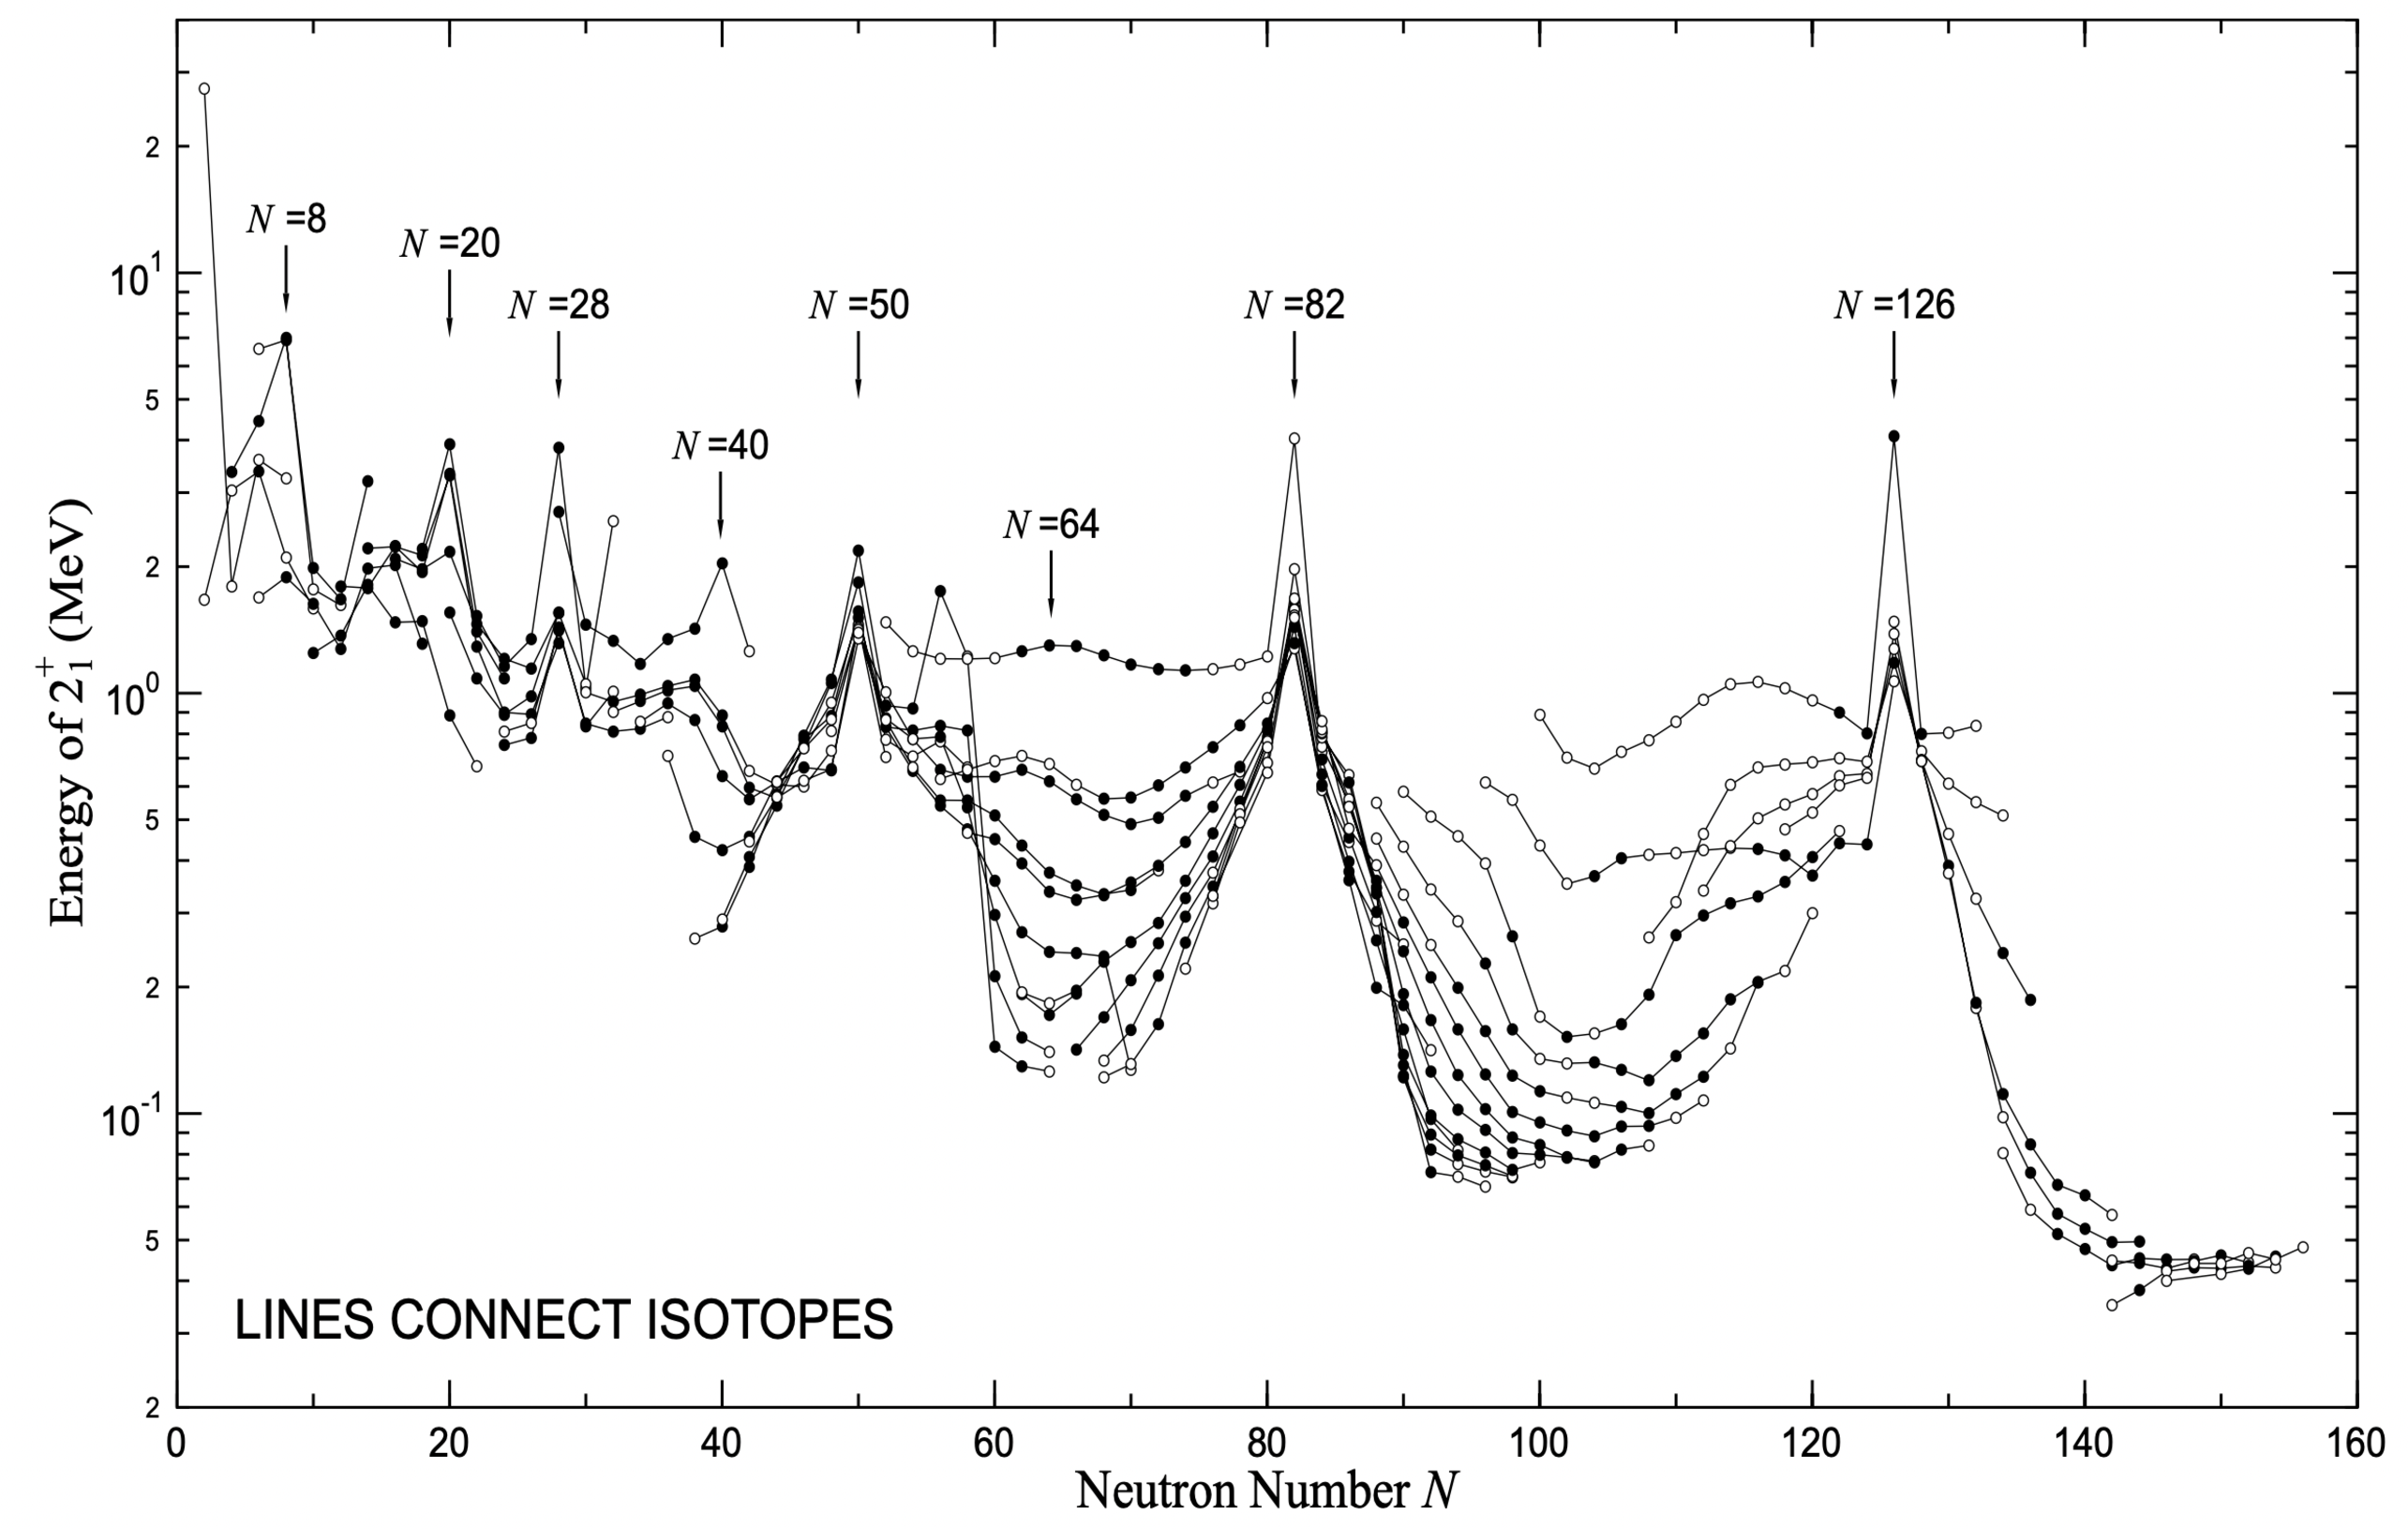
\includegraphics[scale=0.3]{Chapters/Figures/E2plus_neutron.pdf}
    \caption{The first excited energy states $2^+$ of nuclei with even $Z$ and $N$ graphically represented with respect to the neutron number. Each line represents a set of isotopes. Figure taken from Ref. \cite{matta2017exotic}}.
    \label{e2plus_neutron}
\end{figure}

The shell model starts from the basic assumption that the nucleus is a \emph{mean-field potential}, that is a potential for which the motion of a single nucleon is caused by all the other nucleons (the nucleon is moving inside an average potential generated by all the other constituents of the nucleus). Of course, all the nucleons that are under the influence of such a mean field potential occupy the energy levels which correspond to a series of (sub)shells that agree with the Paul exclusion principle. Having a general expression for the potential that properly reproduces all the magic numbers (and the observed nuclear properties) is the main goal.

Since the model starts from the concept of independent (non-interacting) particle motion within an average potential, finding each energy will be equivalent of solving the Schrödinger equation:
\begin{align}
    -\frac{\hbar^2}{2m}\nabla ^2\psi_i(r)+V(r)\psi_i(r)=e_i\psi_i(r)\, 
    \label{schrodinger-single-particle-eq}
\end{align}
where $e_i$ represents the energy (eigenvalue) and $\psi_i$ represents the wave-function (eigenstates), while $V(r)$ is the nuclear potential whose expression must be evaluated.